
\chapter{INTRODUCTION}
\label{chapter:Intro}

%: ----------------------- paths to graphics ------------------------
\ifpdf
    \graphicspath{{1_Introduction/figures/PNG/}{1_Introduction/figures/PDF/}{1_Introduction/figures/}}
\else
    \graphicspath{{1_Introduction/figures/EPS/}{1_Introduction/figures/}}
\fi

% 
%: ----------------------- introduction content -----------------------


This project encompasses aspects of ...............Radar System design can control the rotor position with an accuracy of a micrometer \cite{Cleanroom}. 
\section{Project idea}
\noindent We are considering providing a complete radar system that
will help to reduce the number of accidents on the
highways by implementing a system that is used for car
speed detecting and fast recognizing the detail of the plate
of the car. This system is considered to be better than the
existing road radars and provide new features that will lead
to high accuracy, fast detecting, plate recognition and
plate's details extraction at every radar unit then send the
details to the responsible authority to take the necessary
action with the car driver. This System will meet our
specifications in a simple way with a simple radar circuit
that provide the signal for detecting the cars in an
electromagnetic wave, then make a simple hardware circuit
that provide the speed of the detected car by calibration to
give an order to the camera to picture the over speed cars.
After that the license plate of the car will be extracted from
the car picture and then extract the ARABIC letters and
numbers from the plate, and then send these contents to the
responsible authority by an automatic E-mail. In addition to
that the old system is considered to be expensive (approx
10,000\$) and this system is considered to be maximum
2000\$ and this value is rising according to road type.
\subsection{Main Description:}

\noindent When the car moves in front of the radar circuit, the radar
calculates the car's speed by using the main characteristics of
Doppler frequencies. The output of the radar is voltage varying
from 0 to 50 m volt. Get the output voltage of the radar and turn
it into the ADC circuit to convert it from analogue dc volt form
to digital output, where the computer can deal with it. The
output of the interface will be 8-bits, and then it will vary from 0
to 255.So we need to do our calibration for determining the car's
speed with specific software. After detecting the car speed, we
have to give an order to the camera to capture this car if it
moving over speed and if it's not moving over speed just
determines the speed of it. After taking the photo for the car we
have to does some processing on it to get recognize the license
plate. After recognizing the plates, we extract the information of
the plate and report it.

\subsection*{Project Description}
The radar system is consists of 4 phases:
\begin{itemize}
	\item Radar circuit.
	\item Analogue to digital interface. 
	\item Software's programming for reading the digital input,
	calibration for the car speed, give an order to the camera to
	capture the car. 
	\item Finally the image processing software to recognize the
	plate of the car.
\end{itemize}
\begin{figure}[b]
	\centering
	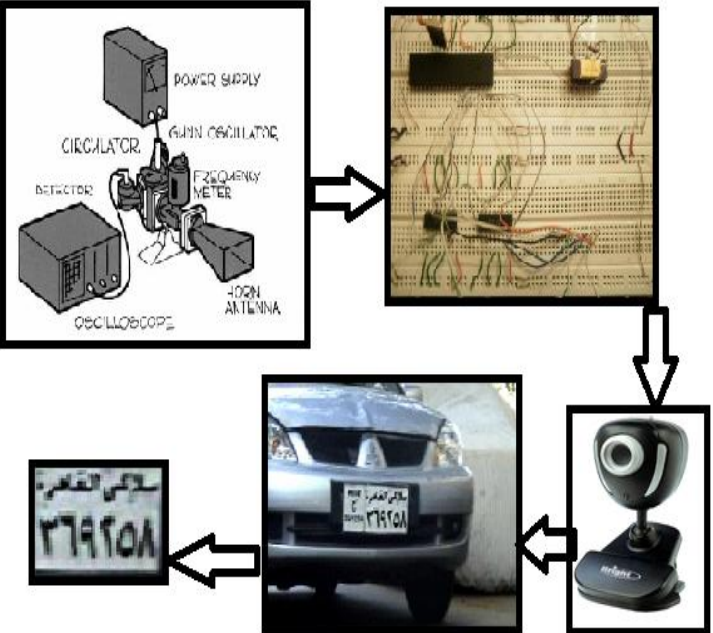
\includegraphics[width=0.45\textwidth]{figure1.png}
\end{figure}

\subsection{Project requirements:}
\begin{itemize}
	\item Information about Radar system.
	\item Radar wave generator circuit.
	\item Analogue to digital interface.
	\item Software for reading from the parallel port.
	\item Software for speed calibration.
	\item Software for image processing and determining the
	plate's contents.
\end{itemize}

\section{Methodology}
\noindent The main goal of this project is to minimize the number of
accidents per years, which occurs all over the roads, by
punishing the drivers that cross the speed limits. So we can
achieve this goal by following some steps to get this
idea.We use the radar to detect a moving car along the road
which the radar will be located. After that by the output of
the radar circuit, we get the output voltage and convert it to
digital form that will be used for measuring the car's speed.
Then the next phase is to order the camera by the input
value of the speed of the car to Taking a photo for the car if
it moving over speed. After saving the image of the car, we
make a number of operations that will be helpful for
analyzing the image, and detect the plate contents to report
it. The last part of the system is to take details of the car's
plate after extract the contents of the plate and sending the
car details to the responsible authority.

\section{Project objectives}
\subsection{HARDWARE \& NETWORK PLATFORMS:}
\noindent We will use for converting from analogue to digital a specific
hardware elements that will help and make it more simple for
implementing the hardware. We will use a microcontroller
for converting from analogue to digital.
\subsection{ Programming Languages:} 
\begin{itemize}
	\item We will use micro C for the program of the
	microcontroler which will be used for analogue
	to digital converter(ADC).
	\item Proteus for circuit simulation.
	\item Csharp and Matlab for inetrface.
	\item Matlab for calibration and license plate
	recognetion(LPR).
\end{itemize}
\subsection{KEY PROJECT BENEFITS:}
\begin{enumerate}
	\item Detect the speeding cars automatically.
	\item Using radar to measure speed of the car to
	avoid accident.
	\item Reduce human element which reduce errors.
	\item Easy handling and low cost.
	\item Make the road safer.
\end{enumerate}
\noindent Now we will speak about each one of the system
componentsto describe every operation in each part and how
it will be connected wih the other phase.
Chapter 2 will be about the radar circuit,its components and
the doppler shift which is the main idea of the radar operation
In chapter 3, chapter 4 we will mention in it how to design
the hardware interface and how it will operate to convert the
output analogue signal from the radar circuit to digital form
to can be easly recognized by the computer by attached the
parallel cable with the interface and the computer.
Chapter 5 will be about when the camera will picture the
moving cars, recognizing informationof the plate of the car
and send these information automaticaly by e-mail to
responsible authority.
At chapter 6 , software engineering is about the flow chart of
the system, constraints and the duration and tasks
implementation.





